% \section{Code testing}
% The code has been designed to be easily tested. The communication and ROS functions are separated from the actual computing of the nodes. 
% \\

% The class structure of the code is hence as follows: the base class performs the operations needed by the node and there exists a wrapper class that implements the publishing and subscribing to the different nodes. \\

% In the actual application, it is an object of this latter wrapper class the one that is created. 
% \\

% This structure easies the testing, since the first testing level is done in the base classes and the second and third on the wrapper classes.
% \\

% For further details about the tools used to perform the testing please read the section \ref{testing}.
% \\

% In the following sections the libraries being tested in each level are presented. 

% 	\subsection{First level: Library unit test}
% 		The library used to perform this unit testing is gtest. More information about that library may be found in the section \ref{gtest}.
% 		In this level, the base classes are tested. Those classes are located in the src/libraries/libraries directory. The tests performed are: 
			% \subsubsection{Converter Test}

			% \subsubsection{ROI Segmenter 2D Test}

			% \subsubsection{ROI Segmenter 3D Test}

			% \subsubsection{Feature Extractor 2D Test}

			% \subsubsection{Feature Extractor 3D Test}

			% \subsubsection{Algorithm2D Test}

			% \subsubsection{Algorithm3D Test}

			% \subsubsection{Event Handler Test}

			% \subsubsection{Data Parser Test}

	% \subsection{Second level: ROS node unit test}
	% 	In order to perform this testing level a library unit test and the rostest tool are needed.The rostest tool is explained in detail in the following \ref{rostest} section.\\

	% 	The tests developed in this level are the following: 

	% \subsection{Third level: ROS node integration / regression test}
	% 	In order to perform a third-level testing, both a unit testing library and the rostest tool are needed. In this project, the tests implemented of this level are the following: 

\vspace{1cm}
\section{Computing performance evaluation}

	This section presents the tests that I performed to evaluate the computing performance of the system. 
	The main objective of these tests is to demonstrate that the system is able to operate in real-time, so it can be used while interacting with a human.
	The topics and the nodes of the system are being evaluated measuring their main characteristics. 
	The nodes computing performance is obtained from their CPU and RAM consumption. 
	The topics are the means of communication of the nodes. 
	In the topics the messages are published and more than one node can subscribe to each topic and hence access to those messages. 
	In this evaluation, the total bandwidth and publishing rate of the topics are measured. 

	% The performance testing is used to benchmark the system.
	% There are different items of the system that are tested. 
	% Since the code is divided in nodes, the performance of each node is evaluated. 
	% The sum of those performances gives the total package benchmarking. 
	% Also, the topics used to communicate the nodes are evaluated. 
	% The details may be found in the sections below. 
	% \\[0.5cm]
	% \begin{itemize}
		% \item{\textbf{Nodes' CPU and RAM usage}}
		% \\
		\subsection{Nodes' CPU and RAM usage}

		The CPU and RAM consumption of each node was measured. 
		The total usage of the whole system can be calculated summing the individual consumptions. 
		In section \ref{results}, the results of this evaluation are presented. 
		The CPU and RAM usage are presented in percentage. 
		% The package developed is composed of different nodes. 
		% Since the computing is distributed, each node has different CPU and RAM usages.
		% That is why in these experiments the particular behavior of each node is evaluated. 
		% The CPU and RAM usages are given in percentages. 
		% The computer used has a i7 processor. 
		% This means that it has four processing cores that uses two threads each, totaling eight virtual cores. 
		% The CPU usage is hence represented from the 0 to the 800\%.
		% The RAM usage is represented from 0 to 100\%.
		% % \\[0.5cm]

		% The whole package benchmarking is obtained summing the performances of the different nodes. 
		% This information is important to know the minimum specifications of the computer used in order to obtain a real-time response of the system.  

		% The results are being shown in section \ref{results} in a table as the one in figure \ref{node_model}.

		% \begin{figure}[H]
		% 		\begin{center}
		% 	    \includegraphics[scale=0.48]{img/tests/node_model.png}
		% 		\caption[Node benchmarking - Table model]{Node benchmarking - Table model}
		% 						\label{node_model}

		% 		\end{center}
		% \end{figure}

\newpage
		% \item{\textbf{Topic network usage}}\\
		\subsection{Topic network usage}

		The computing performance tests also evaluate the topic bandwidth (BW) and frequency requirements. 
		The motivation of this evaluation is the following.
		ROS is a distributed system that allows spreading the computation across multiple machines. 
		This allows to create distributed computing systems where the robots carry low-power consuming computers and delegate the CPU intensive tasks to remote servers.	
		The drawback of this approach is that communicating machines consume network resources. 
		This is specially relevant for image or video tasks, which do consume great amounts of BW. 
		The need to evaluate the BW and frequency requirements of the system comes from this issue. 
		Therefore, the purpose of the topic network usage measurement is to evaluate if the system could be distributed across several machines.
		% The topics communicate the nodes and allow the exchange of information. 
		% The parameters that characterizes the topics are the bandwidth and the publishing frequency.
		% % \paragraph{Bandwidth}\mbox{}\\
		% The bandwidth parameter is the speed at which the data is transmitted. 
		% Its units are kilobytes per second. 
		% The ROS framework has a built-in command that allows to retrieve the maximum, minimum, mean and average bandwidth of a topic. 
		% % The results are presented in a table as the one in figure \ref{topic_bw_model}. 
		% \begin{figure}[H]
		% 		\begin{center}
		% 	    \includegraphics[scale=0.35]{img/tests/topic_bw_model.png}
		% 		\caption[Topic benchmarking - Bandwidth table model]{Topic benchmarking - Bandwidth table model}
		% 		\label{topic_bw_model}
		% 		\end{center}
		% \end{figure}
		% If there are network connectivity problems or rostopic cannot keep up with the publisher, the reported bandwidth might be lower than the actual one. 
		\\

		The publishing frequency of a ROS topic is the number of messages published on it over time. 
		It is measured in Hz. 
		ROS provides a built-in command that is similar to the one above that returns the maximum, minimum and the standard deviation of the time between messages in seconds. 
		Also, it returns the average publishing frequency.  
		% A table like the one in figure \ref{topic_hz_model} is used to present the results.

		% \begin{figure}[H]
		% 		\begin{center}
		% 	    \includegraphics[scale=0.35]{img/tests/topic_hz_model.png}
		% 		\caption[Topic benchmarking - Publishing rate table model]{Topic benchmarking - Publishing rate table model}
		% 						\label{topic_hz_model}
		% 		\end{center}
		% \end{figure}
		% 	\end{itemize}


\section{Evaluation of the object recognition accuracy}
\label{accuracy_experiment}

	This experiment is designed to obtain data related to the accuracy of the system. 
	% In the following sections the conditions and parameters that affect the test are shown and explained as well as the testing procedure that is followed. 
	Sections \ref{setup}, \ref{set_of_objects}, \ref{procedure} and \ref{accuracy_measurement} explain the conditions and parameters that affect the experiment and also the testing procedure that has been followed. 
	%\\[0.5cm]

	% \subsection{Environment \& testing conditions}
		% The test is performed in a room with a crowded background , that is, a room without a blank background and with various objects at different depths.
		% The light source is located behind the RGB-D sensor, directly illuminating the user. 
		% The objects that conform the dataset are located next to the tester to facilitate the accessibility to them. 
	%	The test is performed in a room with uniform background and lightning. 


		%\\%[0.5cm]

	% \begin{figure}[H]
	% 	\begin{center}
	%     \includegraphics[scale=0.3]{img/testing_environment.eps}
	% 	\caption[Testing Environment]{Testing Environment}
	% 	\end{center}
	% \end{figure}

	\subsection{Experimental setup}
	\label{setup}
	The experiment was performed in a highly illuminated room with white walls. 
	The light was a mixture of natural light and artificial light coming from halogens.
	The experiment was performed at a distance of approximately 1.7 m from the RGB-D (Red, Green, Blue and Depth) sensor. 
	The background was composed of a white wall with a painting in the right side, a window in the left side and shelves in the middle-left part. 
	Figure \ref{experimental_setup} presents an sketch of the experimental setup. 

	\begin{figure}[H]
		\begin{center}
	    \includegraphics[scale=0.3]{img/setup.png}
		\caption[Experimental setup sketch]{Experimental setup sketch. }
				\label{experimental_setup}

		\end{center}
	\end{figure}



	\subsection{Experimental set of objects}
	\label{set_of_objects}
		The objects being used in the experiment are common objects. 
		They can be seen in Figure \ref{dataset}.
		Using common objects allow to obtain more reliable experiment results, since they were obtained under working conditions. 
		Common objects are usually featureless. 
		That characteristic complicates the object recognition, since objects with rich textures usually generate more robust descriptors.
		In order to overcome this difficulty, different views of each object are obtained and compared when doing the matching. 
		Also, the introduction of both 2D and 3D features diminish the possibilities of false positives and false negatives. 

		\begin{figure}[H]
				\begin{center}
			    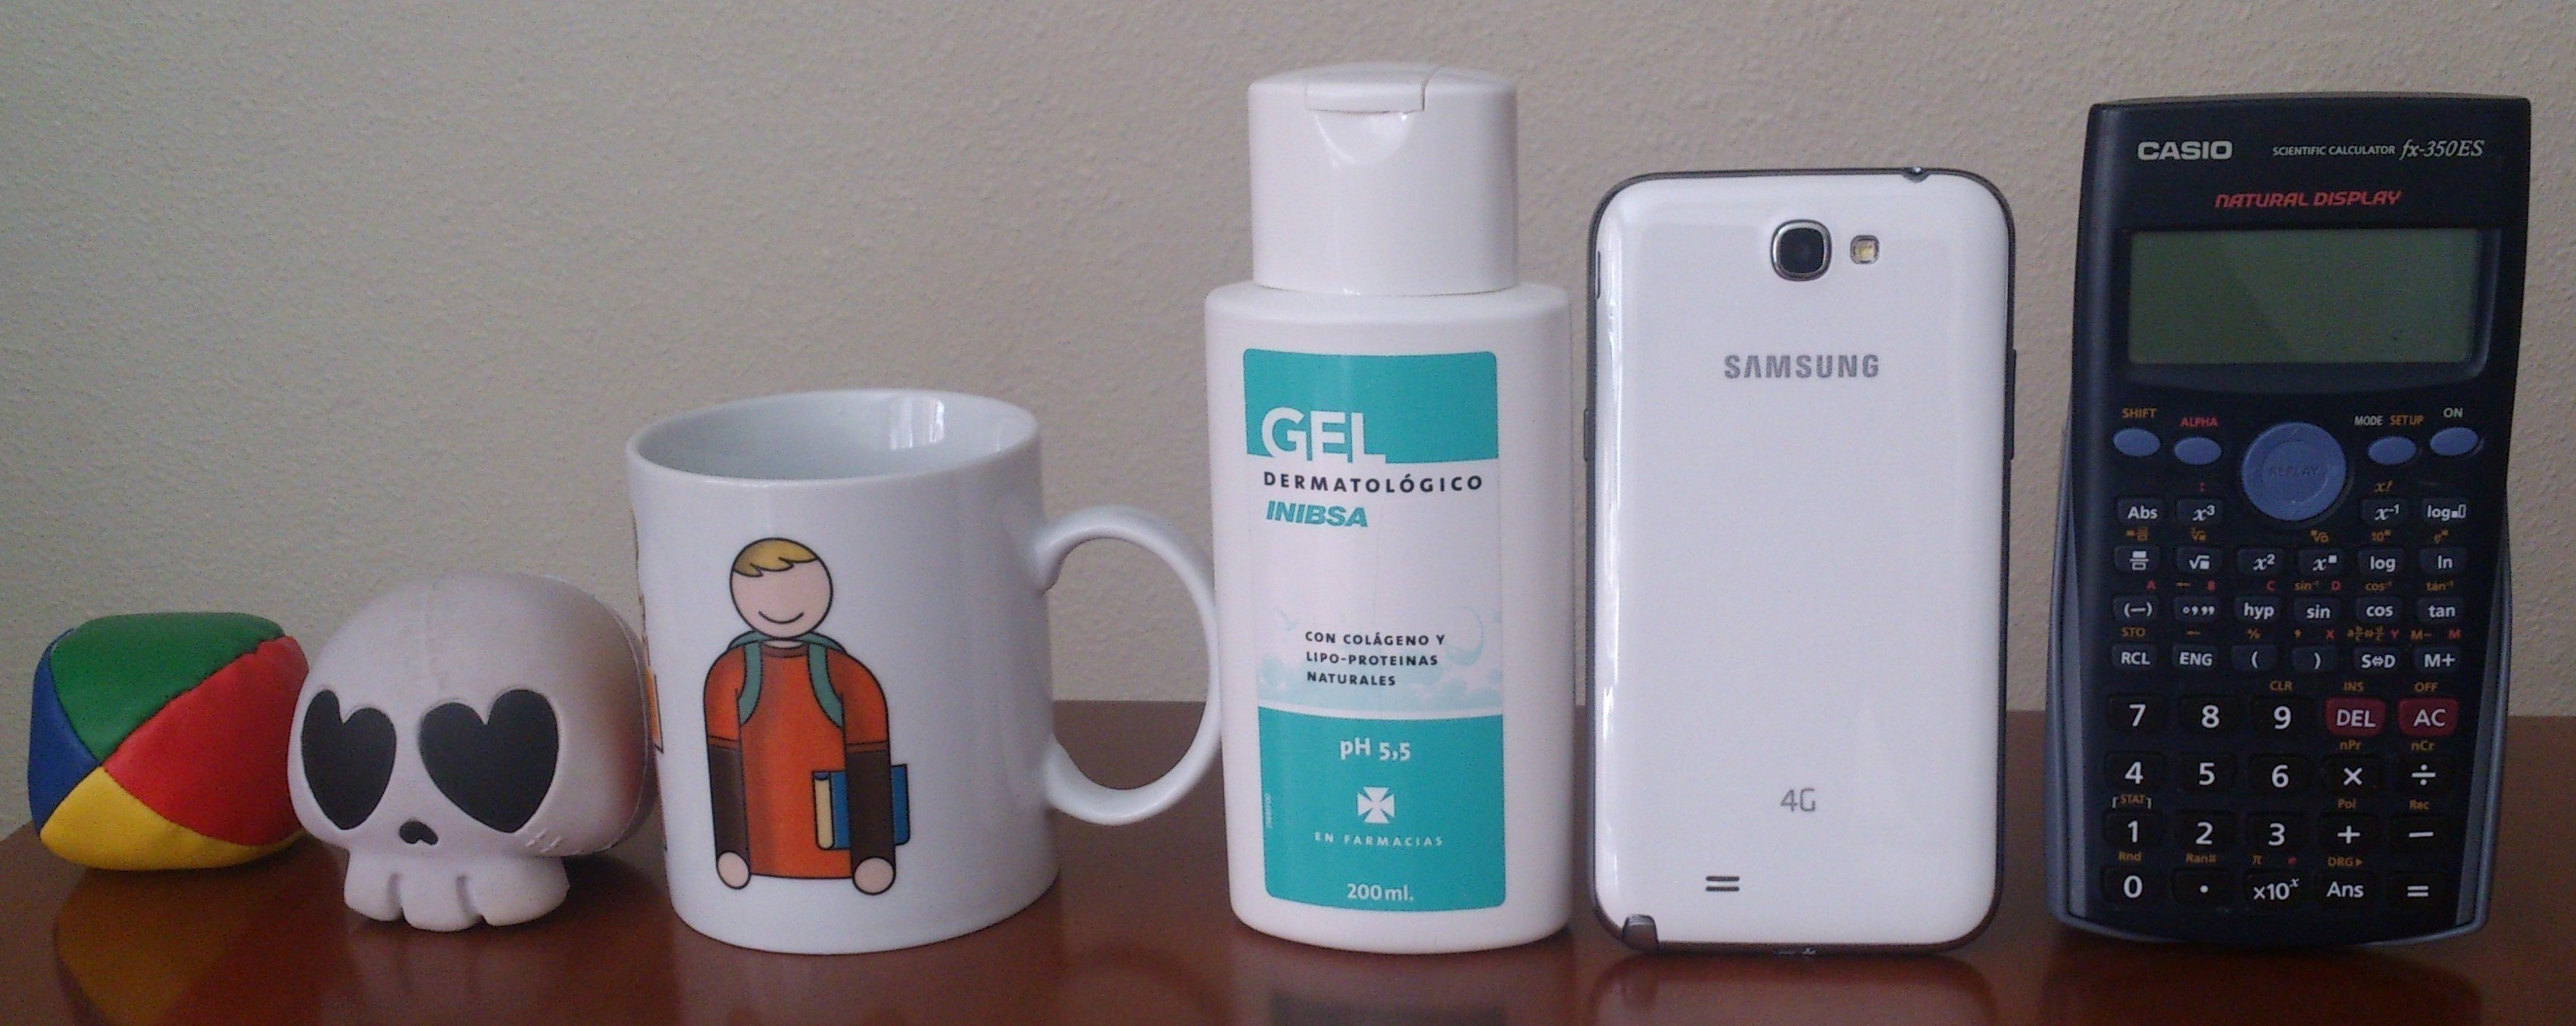
\includegraphics[width=\textwidth]{img/tests/dataset02.jpg}
				\caption[Experimental dataset]{Experimental dataset. From left to right: ball, skull, cup, mobile and calculator.}
				\label{dataset}

				\end{center}
		\end{figure}
	% \subsection{Dataset}


		%This is because the software is intended to be running in a social robot that needs to recognize the most used objects. 
		%Also, the other possible application of the software is as an aiding software for visually impaired persons. 
		%In this case it is a requirement the recognition of daily objects as well.  
		%\\
		% The ones being used in the present experiment may be seen in figure \ref{dataset}. 
	
		This particular dataset is conformed of objects that could be easily confused by a computer vision system using descriptors. 
		As an example, the 3D shape of the ball and the skull is very similar, a fact that would lead to akin 3D descriptors. 
		Also, the cup, the bottle and the mobile have comparable 2D texture. 
		\\%[0.5cm]

	\subsection{Experimental procedure}
	\label{procedure}

		The testing is performed following this sequence. 
		% First, the tester shows the first two objects that are going to be learned. 
		% Afterwards, the recognition mode is tested identifying and storing in a file the output of the matching for both 2D and 3D. 
		% \\
		% Then, another new object is learned and again the recognition is tested. 
		% This sequence is iterated until there are no new objects to be learned. 
		% \\
		% The reason behind this incremental learning is to observe the differences on the effectiveness and the benchmarking of the system when the dataset size changes. 
		% \\
		First, the objects are stored in the program's dataset. 
		In order to do so, each object is recorded using the data acquisition mode of the software. 
		It is done turning the the object in the process in order to obtain as many different views as possible. 
		This improves the performance of the recognition phase when the object is presented in different positions. 
		Afterwards, the recognition mode is used.
		Each of the objects are presented to the system the same amount of time, 30 seconds. 
		The objects are positioned still during 10 seconds in the most natural grasping position. 
		Then, they are rotated during the remaining 20 seconds. 
		This is done to measure the robustness of the system to rotation changes. 
\\

		% It is then when the accuracy of the system is measured. 
		The information about the 2D and 3D separate recognitions and the final software's output is recorded to a file for further processing. 
		That data is presented in chapter \ref{results}.
		The system allows to specify the number of views being taken per object in the data acquisition phase. 
		Taking advantage of this feature, the whole procedure described above is repeated for one, five and ten object views.
		Theoretically, decreasing the number of views should worse the effectiveness of the recognition. %but better the performance of the system, since the processing needed is reduced.
		This experiment is designed to confirm this intuition. 
		\\%[0.5cm]


	% \subsection{Effectiveness measurement}

		% The effectiveness is measured differently for the learning mode than for the recognizing mode. 
		% \\

		% The first mode do not have a possibility of failing in learning, since all the different classes are previously tested and an error on it could only come from a software error. Having this in mind, the effectiveness of this mode is to create the best descriptors possible. 
		% The best descriptor is that one that has a lower size but still is sufficiently robust to allow a good recognition performance. 
		% \\

		% In the case of the second mode, the recognizing, the effectiveness is measured in terms of false negatives and positives versus the true ones. The result is a percentage that indicates how well the features are matched. If the effectiveness is 0\%, the software has a 100\% of false positives and negatives, and if the effectiveness is a 100\%, there is a 100\% of true positives and negatives. 
		% Also, a confusion matrix is constructed using the results of this test in order to offer a visual summary of the performance of the code. 	\\

		% Finally, the F-score or F-measure is computed in order to present the accuracy of the of the system developed in this thesis. 
		\subsection{Accuracy measurement}
		\label{accuracy_measurement}

		The accuracy of the system is measured using the F-score or F-measure. 
		The general formula for a positive real $\beta$ is described in formula \ref{f_beta}. 
		\begin{center}
		\begin{equation}
		\label{f_beta}
		F_\beta=(1+\beta^2)\cdot\frac{precision \cdot recall}{(\beta^2 \cdot precision )+recall}
		\end{equation}
		\end{center}
		% The F-score may be expressed in terms of true and false positives and negatives as shown below: 
		% \\

		% $F_\beta=\frac{(1+\beta^2)\cdot true\_positives}{(1+\beta^2)\cdot true\_positives +\beta^2 \cdot false\_negatives +false\_positives}$
		% \\
		The $\beta$ is a weight whose value depends on the applications of the system being tested. 
		For example, in critical systems such as a police face recognition software it is preferable to have false positives than false negatives.
		Since in this system the weight being given to the precision is the same that the one being given to the recall, $\beta=1$. 
		This special case is called the $F_1 score$, and its formula may be found in equation \ref{f1}.
		The precision and recall are parameters that are described in formulas \ref{precision} and \ref{recall}, respectively. 
	
		
		\begin{center}
		\begin{equation}
		F_1=2\cdot\frac{precision \cdot recall}{precision + recall}
		\label{f1}
		\end{equation}
		\end{center}

		% In this system there is not a special need to give more weight neither to false positives nor false negatives. 
		% Hence, the $F_1 score$ has been chosen as the metric for the accuracy evaluation of the system.		
		Apart from the $F_1 score$, a confusion matrix is constructed for each experiment. 
		This matrix shows the percentage each different object was predicted when each of the real objects were presented to the system. 
		This percentage is shown transformed to a zero to one scale. 
		% \\
		% Usually, confusion matrices present the absolute results but in this case they were converted into ratios in a 0 to 1 range. 
		% When the number of views being learned per object increases, the computing time also is higher and then the number of predicted objects for a same amount of time is lower. 
		% In this experiment, for the 1 view per object experiment, the number of results is larger than the 10 views experiment. 
		% This is the reason why the confusion matrix values are given as a ratio, to construct comparable confusion matrices from each of the experiments. 
		% In this system, each different retrieved a different number of results and hence the matrix is constructed with a ratio from 0 to 1. 
		% The confusion matrix in which the results are being presented is the same as the figure \ref{matrix_model}. 
		% \begin{figure}[H]
		% 		\begin{center}
		% 	    \includegraphics[scale=0.35]{img/tests/matrix_model.png}
		% 		\caption[Confusion matrix model]{Confusion matrix model}
		% 		\label{matrix_model}
		% 		\end{center}
		% \end{figure}
		The precision is the fraction of retrieved results that are relevant.  
		Using a confusion matrix as the one above, the precision is computed from it using formula \ref{precision}.
		\begin{center}
		\begin{equation}
		\label{precision}
		precision_{ij}=\frac{M_{ij}}{\sum M_j}
		\end{equation}
		\end{center}

		$M_{ij}$ are the elements of the confusion matrix. 
		The i represent the rows and the j the columns of the matrix. 
		The recall is the fraction of the results that are relevant and that have succeeded. 
		It may be obtained using the confusion matrix with formula \ref{recall}.
		The precision and recall are computed for each of the six objects conforming the dataset. 

		\begin{center}
		\begin{equation}
		\label{recall}
		recall_{ij}=\frac{M_{ij}}{\sum M_i}
		\end{equation}
		\end{center}
